
\begin{figure}[H]
    \centering



\tikzset{every picture/.style={line width=0.75pt}} %set default line width to 0.75pt        

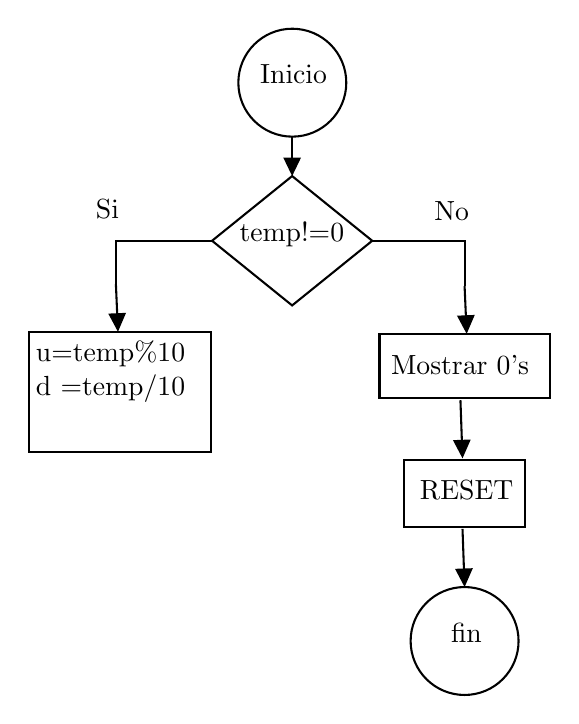
\begin{tikzpicture}[x=0.75pt,y=0.75pt,yscale=-1,xscale=1]
%uncomment if require: \path (0,649); %set diagram left start at 0, and has height of 649

%Flowchart: Connector [id:dp42585090626324207] 
\draw   (300,61) .. controls (300,46.64) and (311.64,35) .. (326,35) .. controls (340.36,35) and (352,46.64) .. (352,61) .. controls (352,75.36) and (340.36,87) .. (326,87) .. controls (311.64,87) and (300,75.36) .. (300,61) -- cycle ;
%Straight Lines [id:da9927818650372262] 
\draw    (325.92,87) -- (325.92,103) ;
\draw [shift={(325.92,106)}, rotate = 270] [fill={rgb, 255:red, 0; green, 0; blue, 0 }  ][line width=0.08]  [draw opacity=0] (8.93,-4.29) -- (0,0) -- (8.93,4.29) -- cycle    ;
%Flowchart: Decision [id:dp8222109791046812] 
\draw   (325.92,106) -- (364.5,137.17) -- (325.92,168.33) -- (287.33,137.17) -- cycle ;
%Shape: Right Angle [id:dp5468713947182464] 
\draw   (287.33,137.17) -- (241,137.17) -- (241,158) ;
%Straight Lines [id:da34123972616362797] 
\draw    (241,158) -- (241.87,178) ;
\draw [shift={(242,181)}, rotate = 267.51] [fill={rgb, 255:red, 0; green, 0; blue, 0 }  ][line width=0.08]  [draw opacity=0] (8.93,-4.29) -- (0,0) -- (8.93,4.29) -- cycle    ;
%Flowchart: Process [id:dp6422094052668206] 
\draw   (199,181) -- (287,181) -- (287,239) -- (199,239) -- cycle ;
%Shape: Right Angle [id:dp9632380337734168] 
\draw   (364.5,137.17) -- (409,137.17) -- (409,159) ;
%Straight Lines [id:da9224648988654192] 
\draw    (409,159) -- (409.87,179) ;
\draw [shift={(410,182)}, rotate = 267.51] [fill={rgb, 255:red, 0; green, 0; blue, 0 }  ][line width=0.08]  [draw opacity=0] (8.93,-4.29) -- (0,0) -- (8.93,4.29) -- cycle    ;
%Flowchart: Process [id:dp38544924804806135] 
\draw   (368,182) -- (450,182) -- (450,213) -- (368,213) -- cycle ;
%Straight Lines [id:da9362534173457413] 
\draw    (407,214) -- (407.89,239) ;
\draw [shift={(408,242)}, rotate = 267.95] [fill={rgb, 255:red, 0; green, 0; blue, 0 }  ][line width=0.08]  [draw opacity=0] (8.93,-4.29) -- (0,0) -- (8.93,4.29) -- cycle    ;
%Flowchart: Process [id:dp015535025341874897] 
\draw   (380,243) -- (438,243) -- (438,275) -- (380,275) -- cycle ;
%Straight Lines [id:da14093121348085114] 
\draw    (408,276) -- (408.89,301) ;
\draw [shift={(409,304)}, rotate = 267.95] [fill={rgb, 255:red, 0; green, 0; blue, 0 }  ][line width=0.08]  [draw opacity=0] (8.93,-4.29) -- (0,0) -- (8.93,4.29) -- cycle    ;
%Flowchart: Connector [id:dp28231580529895073] 
\draw   (383,330) .. controls (383,315.64) and (394.64,304) .. (409,304) .. controls (423.36,304) and (435,315.64) .. (435,330) .. controls (435,344.36) and (423.36,356) .. (409,356) .. controls (394.64,356) and (383,344.36) .. (383,330) -- cycle ;

% Text Node
\draw (309,51) node [anchor=north west][inner sep=0.75pt]   [align=left] {Inicio};
% Text Node
\draw (229.92,116) node [anchor=north west][inner sep=0.75pt]   [align=left] {Si};
% Text Node
\draw (299.08,126.67) node [anchor=north west][inner sep=0.75pt]   [align=left] {temp!=0};
% Text Node
\draw (201,184) node [anchor=north west][inner sep=0.75pt]   [align=left] {u=temp\%10\\d =temp/10};
% Text Node
\draw (392.92,117) node [anchor=north west][inner sep=0.75pt]   [align=left] {No};
% Text Node
\draw (372.08,190.67) node [anchor=north west][inner sep=0.75pt]   [align=left] {Mostrar 0's};
% Text Node
\draw (386,251) node [anchor=north west][inner sep=0.75pt]   [align=left] {RESET};
% Text Node
\draw (401,320) node [anchor=north west][inner sep=0.75pt]   [align=left] {fin};


\end{tikzpicture}

    \caption{Función display}
    \label{FigWW}
\end{figure}
